\let\negmedspace\undefined
\let\negthickspace\undefined
\documentclass[journal]{IEEEtran}
\usepackage[a5paper, margin=10mm, onecolumn]{geometry}
%\usepackage{lmodern} % Ensure lmodern is loaded for pdflatex
\usepackage{tfrupee} % Include tfrupee package

\setlength{\headheight}{1cm} % Set the height of the header box
\setlength{\headsep}{0mm}     % Set the distance between the header box and the top of the text

\usepackage{gvv-book}
\usepackage{gvv}
\usepackage{cite}
\usepackage{amsmath,amssymb,amsfonts,amsthm}
\usepackage{algorithmic}
\usepackage{graphicx}
\usepackage{textcomp}
\usepackage{xcolor}
\usepackage{txfonts}
\usepackage{listings}
\usepackage{enumitem}
\usepackage{mathtools}
\usepackage{gensymb}
\usepackage{comment}
\usepackage[breaklinks=true]{hyperref}
\usepackage{tkz-euclide} 
\usepackage{listings}
% \usepackage{gvv}                                        
\def\inputGnumericTable{}                                 
\usepackage[latin1]{inputenc}                                
\usepackage{color}                                            
\usepackage{array}                                            
\usepackage{longtable}                                       
\usepackage{calc}                                             
\usepackage{multirow}                                         
\usepackage{hhline}                                           
\usepackage{ifthen}                                           
\usepackage{lscape}
\begin{document}

\bibliographystyle{IEEEtran}
\vspace{3cm}
\title{10.4.ex.14.2}
\author{EE24BTECH11025 - GEEDI HARSHA}
% \maketitle
% \newpage
{\let\newpage\relax\maketitle}

\renewcommand{\thefigure}{\theenumi}
\renewcommand{\thetable}{\theenumi}
\setlength{\intextsep}{10pt} % Space between text and floats


\numberwithin{equation}{enumi}
\numberwithin{figure}{enumi}
\renewcommand{\thetable}{\theenumi}



\textbf{Question:}
Formulate the following problem as a pair of equations, and hence find it's solution:

Ritu can row downstream 20 km in 2 hours, and upstream 4 km in 2 hours. Find her speed of rowing in still water and the speed of the current.

\textbf{Solution:}
Let's define:
\begin{align*}
v &= \text{speed in still water} \\
c &= \text{speed of current}
\end{align*}

From given conditions:
\begin{align*}
(v + c) \times 2 &= 20 \\
(v - c) \times 2 &= 4
\end{align*}

Simplifying:
\begin{align*}
v + c &= 10 \\
v - c &= 2
\end{align*}
The above equations can be written in the form $A\vec{x} = \vec{b}$
Where,

\begin{align*}
A &= \begin{pmatrix}
    1 & 1 \\
    1 & -1
    \end{pmatrix} \\
\mathbf{x} &= \begin{pmatrix}
    v \\
    c
    \end{pmatrix} \\
\mathbf{b} &= \begin{pmatrix}
    10 \\
    2
    \end{pmatrix}
\end{align*}

The matrix $A$ can be decomposed into:
\begin{align*}
    A = L \cdot U
\end{align*}

where:
\begin{align*}
    L &= \begin{pmatrix}
    1 & 0 \\
    1 & 1
    \end{pmatrix}, \\
    U &= \begin{pmatrix}
    1 & 1 \\
    0 & -2
    \end{pmatrix}.
\end{align*}

\textbf{Factorization of LU:}
Given a matrix $A$ of size $n \times n$, LU decomposition is performed row by row and column by column. The update equations are as follows:
\begin{enumerate}
    \item Start by initializing $\mathbf{L}$ as the identity matrix $\mathbf{L} = \mathbf{I}$ and $\mathbf{U}$ as a copy of $\mathbf{A}$
    \item For each column $j \geq k$, the entries of $U$ in the $k$-th row are updated as:
    \begin{align*}
        U_{k,j} = A_{k,j} - \sum_{m=1}^{k-1} L_{k,m} \cdot U_{m,j} \quad \forall \quad j \geq k
    \end{align*}
    \item For each row $i > k$, the entries of $L$ in the $k$-th column are updated as:
    \begin{align*}
        L_{i,k} = \frac{1}{U_{k,k}} \left(A_{i,k} - \sum_{m=1}^{k-1} L_{i,m} \cdot U_{m,k}\right) \quad \forall \quad i > k
    \end{align*}
\end{enumerate}

The system $A\mathbf{x} = \mathbf{b}$ is transformed into $L \cdot U \cdot \mathbf{x} = \mathbf{b}$. Let $\mathbf{y}$ satisfy $L\mathbf{y} = \mathbf{b}$:
\begin{align*}
    \begin{pmatrix}
    1 & 0 \\
    1 & 1
    \end{pmatrix}
    \begin{pmatrix}
    y_1 \\
    y_2
    \end{pmatrix} =
    \begin{pmatrix}
    10 \\
    2
    \end{pmatrix}
\end{align*}

Using forward substitution:
\begin{align*}
    y_1 &= 10 \\
    y_1 + y_2 &= 2 \\
    y_2 &= -8
\end{align*}

Thus:
\begin{align*}
    \mathbf{y} = \begin{pmatrix}
    10 \\
    -8
    \end{pmatrix}
\end{align*}

Next, solve $U\mathbf{x} = \mathbf{y}$:
\begin{align*}
    \begin{pmatrix}
    1 & 1 \\
    0 & -2
    \end{pmatrix}
    \begin{pmatrix}
    v \\
    c
    \end{pmatrix} =
    \begin{pmatrix}
    10 \\
    -8
    \end{pmatrix}
\end{align*}

Using backward substitution:
\begin{align*}
    -2c &= -8 \\
    c &= 4 \\
    v + c &= 10 \\
    v &= 6
\end{align*}

Therefore:
\begin{align*}
    \text{Speed in still water } (v) &= 6 \text{ km/h} \\
    \text{Speed of current } (c) &= 4 \text{ km/h}
\end{align*}
\textbf{Alternative Solution using Orthogonal Matrix Properties:}

The system of equations can be written in matrix form $A\mathbf{x} = \mathbf{b}$ where:
\begin{align*}
A &= \begin{pmatrix}
1 & 1 \\
1 & -1
\end{pmatrix}, \\
\mathbf{x} &= \begin{pmatrix}
v \\
c
\end{pmatrix}, \\
\mathbf{b} &= \begin{pmatrix}
10 \\
2
\end{pmatrix}
\end{align*}

Note that matrix $A$ is orthogonal ($A^T \cdot A = I$). Multiplying both sides by $A^T$:
\begin{align*}
A^T A\mathbf{x} &= A^T\mathbf{b} \\
\begin{pmatrix}
1 & 1 \\
1 & -1
\end{pmatrix}
\begin{pmatrix}
1 & 1 \\
1 & -1
\end{pmatrix}
\begin{pmatrix}
v \\
c
\end{pmatrix} &= 
\begin{pmatrix}
1 & 1 \\
1 & -1
\end{pmatrix}
\begin{pmatrix}
10 \\
2
\end{pmatrix}
\end{align*}

This gives:
\begin{align*}
\begin{pmatrix}
2 & 0 \\
0 & 2
\end{pmatrix}
\begin{pmatrix}
v \\
c
\end{pmatrix} &= 
\begin{pmatrix}
12 \\
8
\end{pmatrix}
\end{align*}

Therefore:
\begin{align*}
v &= 6 \text{ km/h} \\
c &= 4 \text{ km/h}
\end{align*}
\begin{figure}[h]
    \centering
    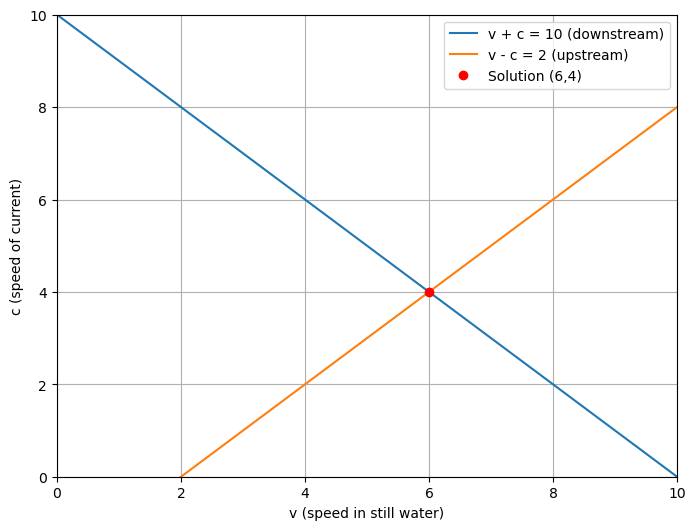
\includegraphics[width=\textwidth]{figs/fig.png}
\end{figure}
\end{document}
